\subsection{Messverfahren}
\paragraph{Untergrundmessung:} Nach Einstellen einer Zählrohr-Betriebsspannug von \(U=\qty{500}{\volt}\) wird die passende Betriebsspannung ermittelt, indem auf das akustische Signal der sprunghaft detektierten Teilchen geachtet wird. Für die Durchführung der Untergrundzählratenmessung \(n_0\) wird anschließend bei einer Messdauer von 5 Minuten die Anzahl der detektierten Zerfälle/Counts gemessen.

\paragraph{Absorption von \(\boldsymbol{\beta}\)-Strahlung:} Die Zerfallstatistik/Zählrate des \ce{^90Sr} Präparats wird für verschiedene Dicken der Aluminiumabschirmung zunächst bei \(\qty{30}{\s}\) und bei kleiner werdenden Zählraten bei entsprechend längeren Messdauer von \(\qty{120}{\s}\) gemessen. Bei ungefährem Erreichen der Untergrundrate wird eine letzte Nulleffektmessung \(n_0^\beta\) bei einer um nochmal einen Millimeter erhöhten Absorberdicke über 5 Minuten durchgeführt. 

\paragraph{Absorption von \(\boldsymbol{\gamma}\)-Strahlung:} Diesmal werden Blei Absorberplatten zur schrittweisen Erhöhung der Absorberdicke benutzt, es wird der Zerfall von \ce{^60Co} über eine Messdauer von \(t=\qty{60}{\s}\) aufgenommen.

\paragraph{Aktivität des \(\boldsymbol{\gamma}\)-Strahlers:} Es wird eine weitere Messreihe bei einem GMZ-Quellen Abstand von \(d=\qtylist{5;10;20}{\cm}\) und \(t=\qty{60}{\s}\) durchgeführt.

\paragraph{Absorptionsmessung und Energiebestimmung von \(\boldsymbol{\alpha}\)-Strahlung:} Die nontrivialste Messung wird mithilfe der Vakuumkammer durchführt: Metallplatten würden Alphastrahlung vollständig abschirmen, sodass ein variabel evakuierbares Glasrohr als Absorber benutzt wird. Feinfühliges Einstellen des Luftdrucks durch Betätigen eines Ventils dient somit der Messung des Zerfalls bei \(t=\qty{60}{\s}\).

\vfill
\subsection{Messprotokoll}
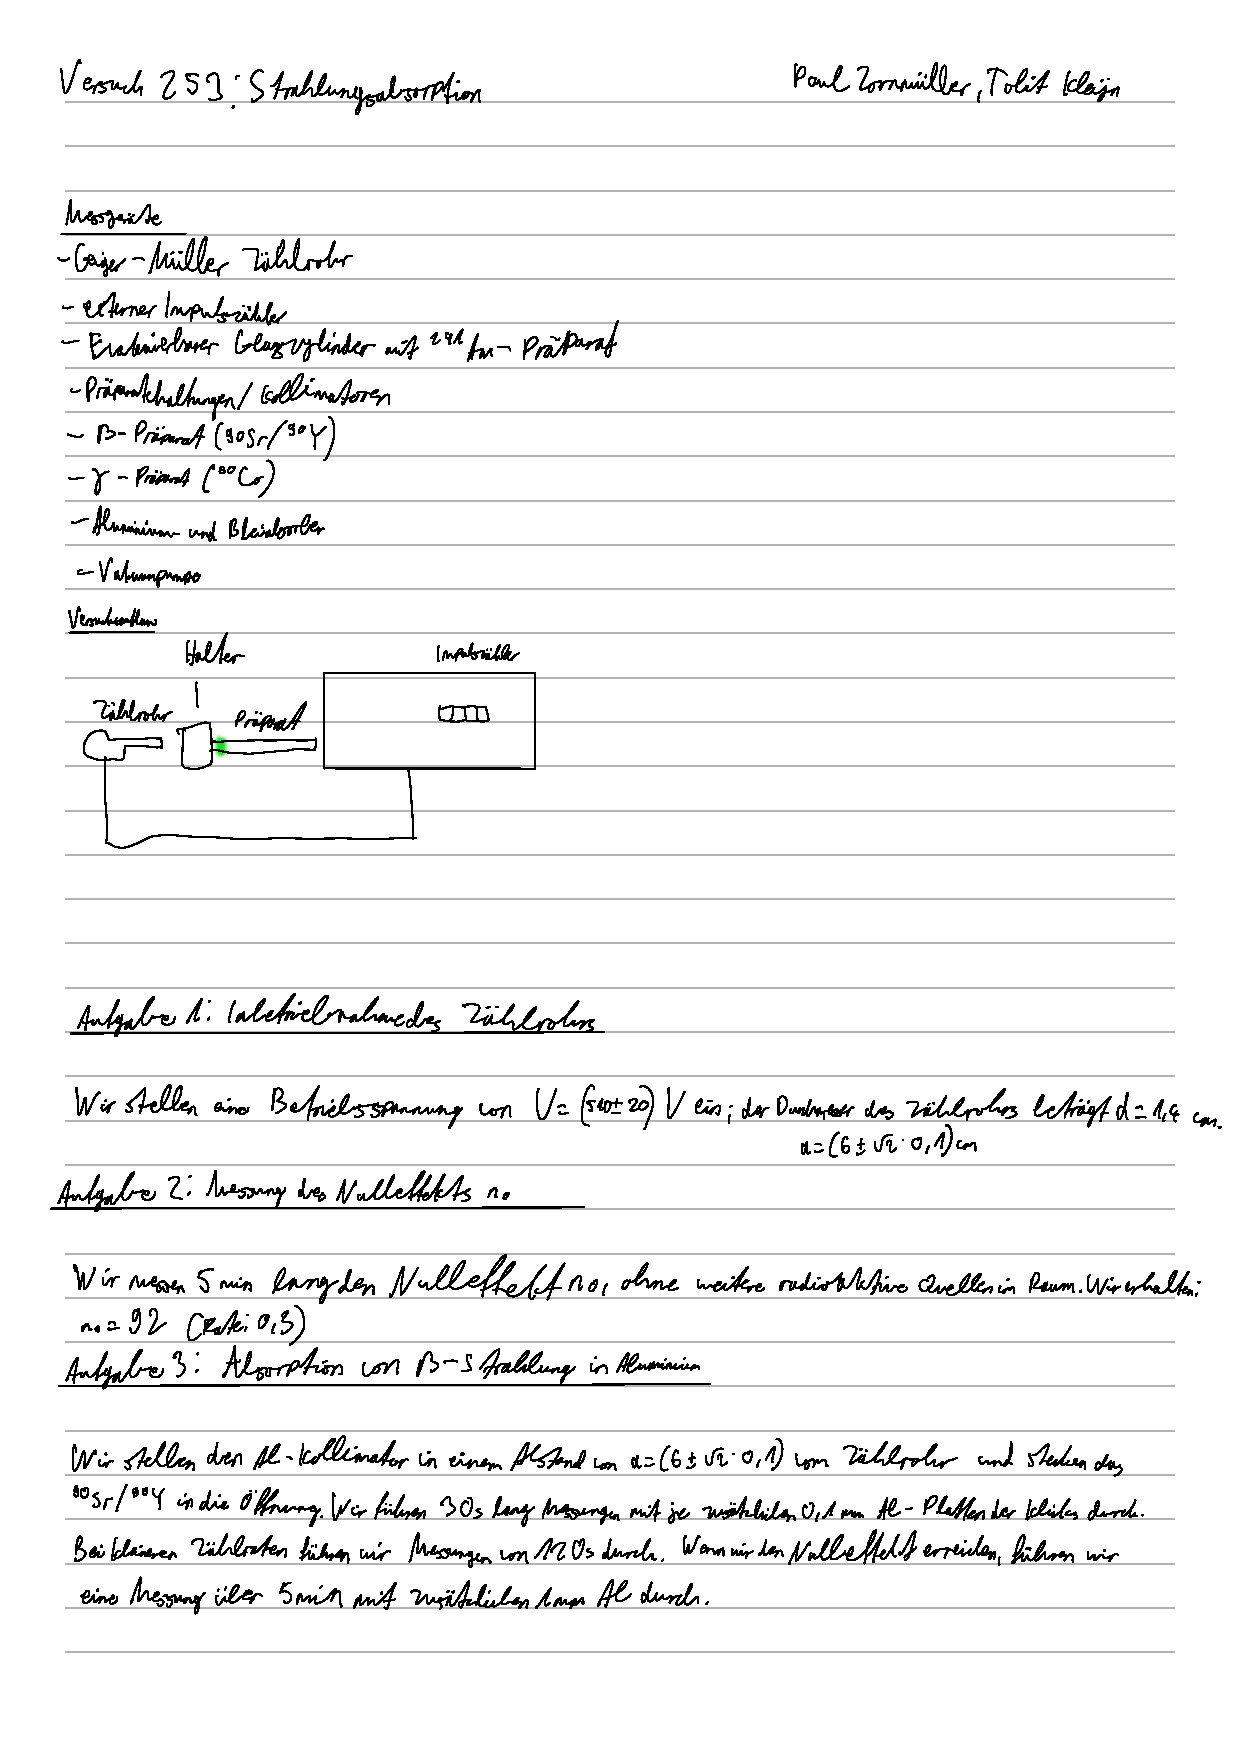
\includepdf[pages=-]{./images/253.pdf}
% heibox.uni-heidelberg.de/d/a48f9d7b91264990a16e/
